\documentclass[a4paper,11pt,final]{article}
% Pour une impression recto verso, utilisez plutôt ce documentclass :
%\documentclass[a4paper,11pt,twoside,final]{article}

%%%%%%%%%%%%%%%%%%%%%%%%%%%%%%%%%%%%%%%%%%%%%%%%%%%%%%%%%%%%%%%%%%%%%%%%%%%%
%   Package
%%%%%%%%%%%%%%%%%%%%%%%%%%%%%%%%%%%%%%%%%%%%%%%%%%%%%%%%%%%%%%%%%%%%%%%%%%%%


\usepackage[english,francais]{babel}
\usepackage[utf8]{inputenc}
\usepackage[T1]{fontenc}
\usepackage[pdftex]{graphicx}
\usepackage{setspace}
\usepackage{hyperref}
\usepackage{epstopdf}
\usepackage[pdftex]{graphicx}
\usepackage{grffile}
\usepackage[french]{varioref}

\usepackage{fancyhdr} % Required for custom headers
\usepackage{lastpage} % Required to determine the last page for the footer
\usepackage{extramarks} % Required for headers and footers
\usepackage{listings} % Required for insertion of code

\usepackage{colortbl} %Clouleur tableau protoypes de fonctions

% Marges
\topmargin=-0.45in
\evensidemargin=0in
\oddsidemargin=0in
\textwidth=6.5in
\textheight=9.0in
\headsep=0.25in

%%%%%%%%%%%%%%%%%%%%%%%%%%%%%%%%%%%%%%%%%%%%%%%%%%%%%%%%%%%%%%%%%%%%%%%%%%%%
%   Info page titre
%%%%%%%%%%%%%%%%%%%%%%%%%%%%%%%%%%%%%%%%%%%%%%%%%%%%%%%%%%%%%%%%%%%%%%%%%%%%

\newcommand{\reporttitle}{Breach, Freak \& Bar Mitzvah : Attaques sur SSL/TLS}     % Titre
\newcommand{\reportauthor}{\textsc{Tremblain} Rémi} % Auteur
\newcommand{\reportsubject}{Projet de fin d'étude} % Sujet
\newcommand{\HRule}{\rule{\linewidth}{0.5mm}}
\setlength{\parskip}{1ex} % Espace entre les paragraphes

\hypersetup{
    pdftitle={\reporttitle},%
    pdfauthor={\reportauthor},%
    pdfsubject={\reportsubject},%
    pdfkeywords={rapport} {SSL} {TLS} {HTTPS}
}

%%%%%%%%%%%%%%%%%%%%%%%%%%%%%%%%%%%%%%%%%%%%%%%%%%%%%%%%%%%%%%%%%%%%%%%%%%%%
%   Mise en place des pieds de page et entêtes
%%%%%%%%%%%%%%%%%%%%%%%%%%%%%%%%%%%%%%%%%%%%%%%%%%%%%%%%%%%%%%%%%%%%%%%%%%%%

\pagestyle{fancy}
\lhead{Tremblain Rémi} % Top left header
\chead{Compte rendu projet} % Top center head
\rhead{Master CSI} % Top right header
\lfoot{\lastxmark} % Bottom left footer
\cfoot{} % Bottom center footer
\rfoot{Page\ \thepage\ sur\ \protect\pageref{LastPage}} % Bottom right footer
\renewcommand\headrulewidth{0.4pt} % Size of the header rule
\renewcommand\footrulewidth{0.4pt} % Size of the footer rule

%%%%%%%%%%%%%%%%%%%%%%%%%%%%%%%%%%%%%%%%%%%%%%%%%%%%%%%%%%%%%%%%%%%%%%%%%%%%
%%%%%%%%%%%%%%%%%%%%%%%%%%%%%%%%%%%%%%%%%%%%%%%%%%%%%%%%%%%%%%%%%%%%%%%%%%%%
%%
%%   Début du document
%%
%%%%%%%%%%%%%%%%%%%%%%%%%%%%%%%%%%%%%%%%%%%%%%%%%%%%%%%%%%%%%%%%%%%%%%%%%%%%%
%%%%%%%%%%%%%%%%%%%%%%%%%%%%%%%%%%%%%%%%%%%%%%%%%%%%%%%%%%%%%%%%%%%%%%%%%%%%

\begin{document}

%%%%%%%%%%%%%%%%%%%%%%%%%%%%%%%%%%%%%%%%%%%%%%%%%%%%%%%%%%%%%%%%%%%%%%%%%%%%
%   Page de titre
%%%%%%%%%%%%%%%%%%%%%%%%%%%%%%%%%%%%%%%%%%%%%%%%%%%%%%%%%%%%%%%%%%%%%%%%%%%%
%\begin{titlepage}

\begin{center}

\begin{minipage}[t]{0.48\textwidth}
  \begin{flushleft}
    
\includegraphics [width=80mm]{images/logo-univ.jpg} \\[0.5cm]
    \begin{spacing}{1.5}
      \textsc{\LARGE Université de Bordeaux}
    \end{spacing}
  \end{flushleft}
\end{minipage} \\[1.5cm]

\textsc{\Large \reportsubject}\\[0.5cm]
\HRule \\[0.4cm]
{\huge \bfseries \reporttitle}\\[0.4cm]
\HRule \\[1.5cm]

\begin{minipage}[t]{0.3\textwidth}
  \begin{flushleft} \large
    \emph{Auteur :}\\
    \reportauthor
  \end{flushleft}
\end{minipage}
\begin{minipage}[t]{0.6\textwidth}
  \begin{flushright} \large
    \emph{Responsable :} \\
    M.~Abdel \textsc{Guermouche} \\
  \end{flushright}
\end{minipage}

\vfill

{\large 25 janvier 2016}

\end{center}

\end{titlepage}


\begin{titlepage}

\begin{center}

\begin{minipage}[t]{0.48\textwidth}
  \begin{flushleft}
    
\includegraphics [width=80mm]{images/logo-univ.jpg} \\[0.5cm]
    \begin{spacing}{1.5}
      \textsc{\LARGE Université de Bordeaux}
    \end{spacing}
  \end{flushleft}
\end{minipage} \\[3.5cm]

\textsc{\Large \reportsubject}\\[0.5cm]
\HRule \\[0.4cm]
{\huge \bfseries \reporttitle}\\[0.4cm]
\HRule \\[1.5cm]

\begin{minipage}[t]{0.3\textwidth}
  \begin{flushleft} \large
    \emph{Auteur :}\\
    \reportauthor
  \end{flushleft}
\end{minipage}
\begin{minipage}[t]{0.6\textwidth}
  \begin{flushright} \large
    \emph{Responsable :} \\
    M.~Abdel \textsc{Guermouche} \\
  \end{flushright}
\end{minipage}

\vfill

{\large 25 janvier 2016}

\end{center}

\end{titlepage}
\cleardoublepage % Dans le cas du recto verso, ajoute une page blanche si besoin

%%%%%%%%%%%%%%%%%%%%%%%%%%%%%%%%%%%%%%%%%%%%%%%%%%%%%%%%%%%%%%%%%%%%%%%%%%%%
%   Sommaire
%%%%%%%%%%%%%%%%%%%%%%%%%%%%%%%%%%%%%%%%%%%%%%%%%%%%%%%%%%%%%%%%%%%%%%%%%%%%

\tableofcontents % Table des matières
\sloppy          % Justification moins stricte : des mots ne dépasseront pas des paragraphes
\cleardoublepage
 
%%%%%%%%%%%%%%%%%%%%%%%%%%%%%%%%%%%%%%%%%%%%%%%%%%%%%%%%%%%%%%%%%%%%%%%%%%%%
%   Remerciement
%%%%%%%%%%%%%%%%%%%%%%%%%%%%%%%%%%%%%%%%%%%%%%%%%%%%%%%%%%%%%%%%%%%%%%%%%%%%
%\section*{Remerciements}
\addcontentsline{toc}{section}{Remerciements}

Je tiens à remercier \LaTeX{} et les tutoriels sur internet et notamment \url{http://www.ukonline.be/programmation/latex/tutoriel/index.php}.

Bla bla bla bla bla.

\section*{Remerciements}
\addcontentsline{toc}{section}{Remerciements}

Je tiens à remercier \LaTeX{} et les tutoriels sur internet et notamment \url{http://www.ukonline.be/programmation/latex/tutoriel/index.php}.

Bla bla bla bla bla.

\cleardoublepage


%%%%%%%%%%%%%%%%%%%%%%%%%%%%%%%%%%%%%%%%%%%%%%%%%%%%%%%%%%%%%%%%%%%%%%%%%%%%
%   Introduction
%%%%%%%%%%%%%%%%%%%%%%%%%%%%%%%%%%%%%%%%%%%%%%%%%%%%%%%%%%%%%%%%%%%%%%%%%%%%
%\chapter*{Introduction}

Lorem ipsum dolor sit amet, consectetur adipiscing elit. Fusce luctus
euismod nunc, quis tincidunt lorem egestas in. Nulla hendrerit vel
ante eu gravida. Vivamus eu dapibus libero. Vestibulum dolor tortor,
malesuada et leo et, luctus faucibus augue. Nullam dapibus, tortor non
vulputate rutrum, dolor risus posuere ligula, a tincidunt sapien velit
non odio. Pellentesque sit amet aliquet augue. Nam interdum nunc non
ornare dapibus. Aliquam congue vitae sapien non rutrum. Vestibulum
varius iaculis luctus. Donec vitae congue est. Nunc mattis libero sed
nisl vestibulum, ut vestibulum leo aliquet. Donec volutpat arcu
cursus, varius nunc sit amet, elementum mauris. Aenean auctor
facilisis ultrices. Nulla et magna mi. Ut pretium lacus et risus
tempor cursus.

 Cras sed magna ut nunc varius ornare. Sed sollicitudin porttitor
 metus, nec dignissim neque egestas non. Vestibulum suscipit
 sollicitudin pellentesque. Vivamus vehicula mauris faucibus fermentum
 viverra. Donec ac risus nec magna molestie ornare eu quis metus.
 Nulla eu erat quis mi eleifend volutpat et eu justo. Proin id ipsum
 in purus pellentesque tempor. Maecenas tristique tincidunt elit, quis
 rhoncus velit lobortis eu. Nunc sit amet nisi vehicula, varius massa
 nec, pellentesque nulla. Fusce porta mi ut vulputate vulputate. Fusce
 sed ornare tortor, gravida fermentum nibh.

Nullam imperdiet purus at arcu pretium faucibus. Quisque bibendum
velit enim, eu volutpat mauris lacinia sit amet. Nulla dictum posuere
urna sed tincidunt. Mauris eget lobortis turpis, vitae consequat
turpis. Pellentesque habitant morbi tristique senectus et netus et
malesuada fames ac turpis egestas. Etiam at dui ut neque accumsan
tempus. Suspendisse vitae dolor placerat, adipiscing nunc sit amet,
consectetur elit. Nam euismod augue eu consequat faucibus. Vivamus
rhoncus lorem fringilla quam sagittis, in facilisis ante ultrices.
Praesent elementum augue non odio pellentesque, eget euismod justo
volutpat. Integer convallis dignissim orci ac varius. Aenean cursus
metus vel risus fringilla cursus. Fusce vitae gravida nibh, semper
fringilla leo. Pellentesque lorem nunc, vehicula ut sapien et,
hendrerit luctus sem.

Nam nulla sapien, fermentum in lectus eu, rhoncus feugiat tortor. Sed
et arcu quis nibh egestas ultrices. Sed eu blandit libero. Suspendisse
et ultricies purus. Interdum et malesuada fames ac ante ipsum primis
in faucibus. Sed viverra, urna a adipiscing tristique, augue orci
ornare tellus, sed cursus mauris lacus sit amet magna. Integer
hendrerit laoreet tincidunt. Pellentesque varius condimentum purus ac
interdum. Nullam quam tortor, suscipit at porta in, laoreet nec nulla.
Ut varius ligula enim, in feugiat erat malesuada vitae. Nunc ligula
elit, iaculis nec lobortis eu, accumsan a justo. Maecenas volutpat
laoreet lorem. Phasellus fringilla lacus et dui fermentum sagittis.
Morbi vitae leo eget neque gravida egestas. Mauris dolor metus,
consectetur nec ultricies at, egestas quis ligula. Proin mollis nec
purus eget sollicitudin.

Sed quis ante ac quam semper pretium vitae at urna. Ut id mollis dui.
Duis venenatis ante vel justo lobortis laoreet. Nulla facilisi. Cras
massa massa, tristique cursus mattis non, luctus sed tellus. Morbi in
dui bibendum orci consequat gravida. Vestibulum sed augue et odio
posuere vehicula a ac odio. Ut eleifend, purus eget volutpat
tincidunt, orci ante malesuada dui, quis scelerisque metus dolor et
metus. Phasellus volutpat hendrerit egestas.

Aenean eget mollis nisl, eu varius magna. Vestibulum bibendum dui ut
odio eleifend sodales. Maecenas sollicitudin erat eget erat facilisis,
quis condimentum orci ultrices. Mauris ullamcorper nisl ut augue
ultricies elementum. Integer ullamcorper tortor sit amet condimentum
varius. Aenean venenatis porta urna, nec sollicitudin turpis
ullamcorper quis. Curabitur auctor tristique felis in porta. Nullam a
vestibulum orci. Integer ultrices turpis vitae augue congue, a pretium
elit volutpat. Aliquam semper, tellus dignissim viverra vulputate,
lectus augue suscipit mi, vitae hendrerit augue lectus eu mi. Vivamus
eu orci felis. Sed sollicitudin sapien sed turpis malesuada blandit.
Cras ultrices blandit velit vel sodales. Vivamus consectetur facilisis
ante sit amet dapibus.


\section*{Introduction} % Pas de numérotation
\addcontentsline{toc}{section}{Introduction} % Ajout dans la table des matières

SL/TLS est un des standards les plus répandus pour la securisation des communications sur internet. Bien que le protocole soit assez simple et robuste, de nombreuses attaques ont été mises au point pour récupérer le contenu en clair des communications. Une premiere étape de ce projet consistera donc à faire un inventaire des diffé- rentes techniques existantes visant à attaquer SSL/TLS. Puis dans un second temps, on s’intéressera aux dernieres en date, à savoir Breach, Freak et Bar Mitzvah. Ces attaques, bien qu’assez complexes, permettent d’attaquer une communication http securisée via SSL/TLS (https) pour récuperer des informations sensibles en clair (en l’occurrence les cookies d’authentification). L’objectif sera d’étudier ces attaques de manière assez fine et de les mettre en œuvre (dans la mesure du possible pour ce qui est de Breach et Bar Mitzvah).

\cleardoublepage

%%%%%%%%%%%%%%%%%%%%%%%%%%%%%%%%%%%%%%%%%%%%%%%%%%%%%%%%%%%%%%%%%%%%%%%%%%%%
%  Section
%%%%%%%%%%%%%%%%%%%%%%%%%%%%%%%%%%%%%%%%%%%%%%%%%%%%%%%%%%%%%%%%%%%%%%%%%%%%
%\section{La première section}


\subsection{Une sous section}

On peut mettre des mots en \emph{italique}, 
en \textsc{petites Majuscules} ou 
en \texttt{largeur fixe (machine à écrire)}.

Voici un deuxième paragraphe avec une formule mathématique simple : $e = mc^2$.

Un troisième avec des \og guillemet français \fg{}.

\subsubsection{Écrire en anglais}

\foreignlanguage{english}{Do you speak French? Does anybody here speak french?}


\subsection{Lites}

\begin{itemize}
\item Liste classique ;
\item un élément ;
\item et un autre élément.
\end{itemize}
\vspace{\parskip} % espace entre paragraphes

\begin{enumerate}
\item Une liste numéroté
\item deux
\item trois
\end{enumerate}
\vspace{\parskip}

\begin{description}
\item[Description] C'est bien pour des définitions.
\item[Deux] Ou pour faire un liste spéciale.
\end{description}
\vspace{\parskip}


\subsection{Références}

%Voici une référence à l'image de la figure \ref{bloghiko} page \pageref{bloghiko} et une autre vers la partie \ref{p2} page \pageref{p2}.

%On peut citer un livre\,\up{\cite{lpp}} et on précise les détails à la fin du rapport dans la partie références.


\subsection{Note de bas de page}

Voici une note\,\footnote{Texte de bas de page} de bas de page.
Une deuxième\,\footnotemark{} déclarée différemment.
La même note\,\footnotemark[\value{footnote}].

\footnotetext{Il a deux références vers cette note}


\subsection{Figure}

\begin{figure}[!ht]
    \center
    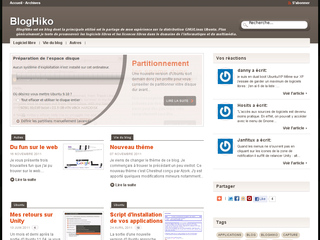
\includegraphics[]{./images/bloghiko.jpg}
    \caption{BlogHiko | taille original}
    \label{bloghiko}
\end{figure}

\begin{figure}[!ht]
    \center
    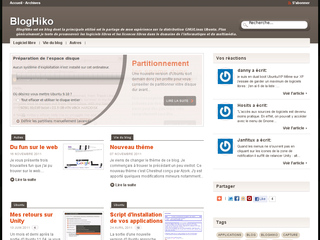
\includegraphics[width=0.5\textwidth]{./images/bloghiko.jpg}
    \caption{BlogHiko | 50\% de la largeur de la page}
\end{figure}



  
\section{La première section}


\subsection{Une sous section}

On peut mettre des mots en \emph{italique}, 
en \textsc{petites Majuscules} ou 
en \texttt{largeur fixe (machine à écrire)}.

Voici un deuxième paragraphe avec une formule mathématique simple : $e = mc^2$.

Un troisième avec des \og guillemet français \fg{}.

\subsubsection{Écrire en anglais}

\foreignlanguage{english}{Do you speak French? Does anybody here speak french?}


\subsection{Lites}

\begin{itemize}
\item Liste classique ;
\item un élément ;
\item et un autre élément.
\end{itemize}
\vspace{\parskip} % espace entre paragraphes

\begin{enumerate}
\item Une liste numéroté
\item deux
\item trois
\end{enumerate}
\vspace{\parskip}

\begin{description}
\item[Description] C'est bien pour des définitions.
\item[Deux] Ou pour faire un liste spéciale.
\end{description}
\vspace{\parskip}


\subsection{Références}

%Voici une référence à l'image de la figure \ref{bloghiko} page \pageref{bloghiko} et une autre vers la partie \ref{p2} page \pageref{p2}.

%On peut citer un livre\,\up{\cite{lpp}} et on précise les détails à la fin du rapport dans la partie références.


\subsection{Note de bas de page}

Voici une note\,\footnote{Texte de bas de page} de bas de page.
Une deuxième\,\footnotemark{} déclarée différemment.
La même note\,\footnotemark[\value{footnote}].

\footnotetext{Il a deux références vers cette note}


\subsection{Figure}

\begin{figure}[!ht]
    \center
    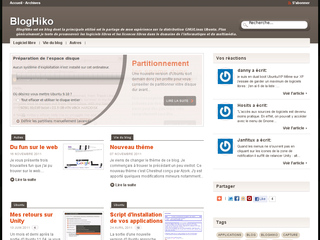
\includegraphics[]{./images/bloghiko.jpg}
    \caption{BlogHiko | taille original}
    \label{bloghiko}
\end{figure}

\begin{figure}[!ht]
    \center
    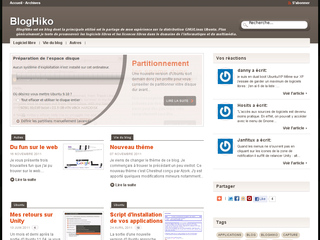
\includegraphics[width=0.5\textwidth]{./images/bloghiko.jpg}
    \caption{BlogHiko | 50\% de la largeur de la page}
\end{figure}

\cleardoublepage

\section{Citation Wikipédia}
\label{p2}


LaTeX est un langage et un système de composition de documents créé par Leslie Lamport en 198312. Plus exactement, il s'agit d'une collection de macro-commandes destinées à faciliter l'utilisation du \og processeur de texte \fg{} TeX de Donald Knuth. Depuis 1993, il est maintenu par le LaTeX3 Project team. La première version utilisée largement, appelée LaTeX2.09, est sortie en 1984. Une révision majeure, appelée LaTeX2 epsilon est sortie en 1991.

Le nom est l'abréviation de Lamport TeX. On écrit souvent \LaTeX, le logiciel permettant les mises en forme correspondant au logo.

Du fait de sa relative simplicité, il est devenu la méthode privilégiée d'écriture de documents scientifiques employant TeX. Il est particulièrement utilisé dans les domaines techniques et scientifiques pour la production de documents de taille moyenne ou importante (thèse ou livre, par exemple). Néanmoins, il peut aussi être employé pour générer des documents de types variés (par exemple, des lettres, ou des transparents).

\cleardoublepage

%%%%%%%%%%%%%%%%%%%%%%%%%%%%%%%%%%%%%%%%%%%%%%%%%%%%%%%%%%%%%%%%%%%%%%%%%%%%
%   Conclusion
%%%%%%%%%%%%%%%%%%%%%%%%%%%%%%%%%%%%%%%%%%%%%%%%%%%%%%%%%%%%%%%%%%%%%%%%%%%%
%\chapter*{Conclusion}

Lorem ipsum dolor sit amet, consectetur adipiscing elit. Fusce luctus
euismod nunc, quis tincidunt lorem egestas in. Nulla hendrerit vel
ante eu gravida. Vivamus eu dapibus libero. Vestibulum dolor tortor,
malesuada et leo et, luctus faucibus augue. Nullam dapibus, tortor non
vulputate rutrum, dolor risus posuere ligula, a tincidunt sapien velit
non odio. Pellentesque sit amet aliquet augue. Nam interdum nunc non
ornare dapibus. Aliquam congue vitae sapien non rutrum. Vestibulum
varius iaculis luctus. Donec vitae congue est. Nunc mattis libero sed
nisl vestibulum, ut vestibulum leo aliquet. Donec volutpat arcu
cursus, varius nunc sit amet, elementum mauris. Aenean auctor
facilisis ultrices. Nulla et magna mi. Ut pretium lacus et risus
tempor cursus.

 Cras sed magna ut nunc varius ornare. Sed sollicitudin porttitor
 metus, nec dignissim neque egestas non. Vestibulum suscipit
 sollicitudin pellentesque. Vivamus vehicula mauris faucibus fermentum
 viverra. Donec ac risus nec magna molestie ornare eu quis metus.
 Nulla eu erat quis mi eleifend volutpat et eu justo. Proin id ipsum
 in purus pellentesque tempor. Maecenas tristique tincidunt elit, quis
 rhoncus velit lobortis eu. Nunc sit amet nisi vehicula, varius massa
 nec, pellentesque nulla. Fusce porta mi ut vulputate vulputate. Fusce
 sed ornare tortor, gravida fermentum nibh.

Nullam imperdiet purus at arcu pretium faucibus. Quisque bibendum
velit enim, eu volutpat mauris lacinia sit amet. Nulla dictum posuere
urna sed tincidunt. Mauris eget lobortis turpis, vitae consequat
turpis. Pellentesque habitant morbi tristique senectus et netus et
malesuada fames ac turpis egestas. Etiam at dui ut neque accumsan
tempus. Suspendisse vitae dolor placerat, adipiscing nunc sit amet,
consectetur elit. Nam euismod augue eu consequat faucibus. Vivamus
rhoncus lorem fringilla quam sagittis, in facilisis ante ultrices.
Praesent elementum augue non odio pellentesque, eget euismod justo
volutpat. Integer convallis dignissim orci ac varius. Aenean cursus
metus vel risus fringilla cursus. Fusce vitae gravida nibh, semper
fringilla leo. Pellentesque lorem nunc, vehicula ut sapien et,
hendrerit luctus sem.

Nam nulla sapien, fermentum in lectus eu, rhoncus feugiat tortor. Sed
et arcu quis nibh egestas ultrices. Sed eu blandit libero. Suspendisse
et ultricies purus. Interdum et malesuada fames ac ante ipsum primis
in faucibus. Sed viverra, urna a adipiscing tristique, augue orci
ornare tellus, sed cursus mauris lacus sit amet magna. Integer
hendrerit laoreet tincidunt. Pellentesque varius condimentum purus ac
interdum. Nullam quam tortor, suscipit at porta in, laoreet nec nulla.
Ut varius ligula enim, in feugiat erat malesuada vitae. Nunc ligula
elit, iaculis nec lobortis eu, accumsan a justo. Maecenas volutpat
laoreet lorem. Phasellus fringilla lacus et dui fermentum sagittis.
Morbi vitae leo eget neque gravida egestas. Mauris dolor metus,
consectetur nec ultricies at, egestas quis ligula. Proin mollis nec
purus eget sollicitudin.

Sed quis ante ac quam semper pretium vitae at urna. Ut id mollis dui.
Duis venenatis ante vel justo lobortis laoreet. Nulla facilisi. Cras
massa massa, tristique cursus mattis non, luctus sed tellus. Morbi in
dui bibendum orci consequat gravida. Vestibulum sed augue et odio
posuere vehicula a ac odio. Ut eleifend, purus eget volutpat
tincidunt, orci ante malesuada dui, quis scelerisque metus dolor et
metus. Phasellus volutpat hendrerit egestas.

Aenean eget mollis nisl, eu varius magna. Vestibulum bibendum dui ut
odio eleifend sodales. Maecenas sollicitudin erat eget erat facilisis,
quis condimentum orci ultrices. Mauris ullamcorper nisl ut augue
ultricies elementum. Integer ullamcorper tortor sit amet condimentum
varius. Aenean venenatis porta urna, nec sollicitudin turpis
ullamcorper quis. Curabitur auctor tristique felis in porta. Nullam a
vestibulum orci. Integer ultrices turpis vitae augue congue, a pretium
elit volutpat. Aliquam semper, tellus dignissim viverra vulputate,
lectus augue suscipit mi, vitae hendrerit augue lectus eu mi. Vivamus
eu orci felis. Sed sollicitudin sapien sed turpis malesuada blandit.
Cras ultrices blandit velit vel sodales. Vivamus consectetur facilisis
ante sit amet dapibus.


\section*{Conclusion}

\addcontentsline{toc}{section}{Conclusion}

Pour conclure, avec \LaTeX{} on obtient un rendu impeccable mais il faut s'investir pour le prendre en main.

\cleardoublepage

%%%%%%%%%%%%%%%%%%%%%%%%%%%%%%%%%%%%%%%%%%%%%%%%%%%%%%%%%%%%%%%%%%%%%%%%%%%%
%   Réference
%%%%%%%%%%%%%%%%%%%%%%%%%%%%%%%%%%%%%%%%%%%%%%%%%%%%%%%%%%%%%%%%%%%%%%%%%%%%
%\phantomsection\addcontentsline{toc}{section}{Références}
\begin{thebibliography}{ABC}	
    \bibitem[REF]{reference} auteur. \emph{titre}. édition, année.
    \bibitem[LPP]{lpp} Rolland. \emph{LaTeX par la pratique}. O'Reilly, 1999.
\end{thebibliography}



\end{document}

